\section{Overview}


\begin{figure}[h]
  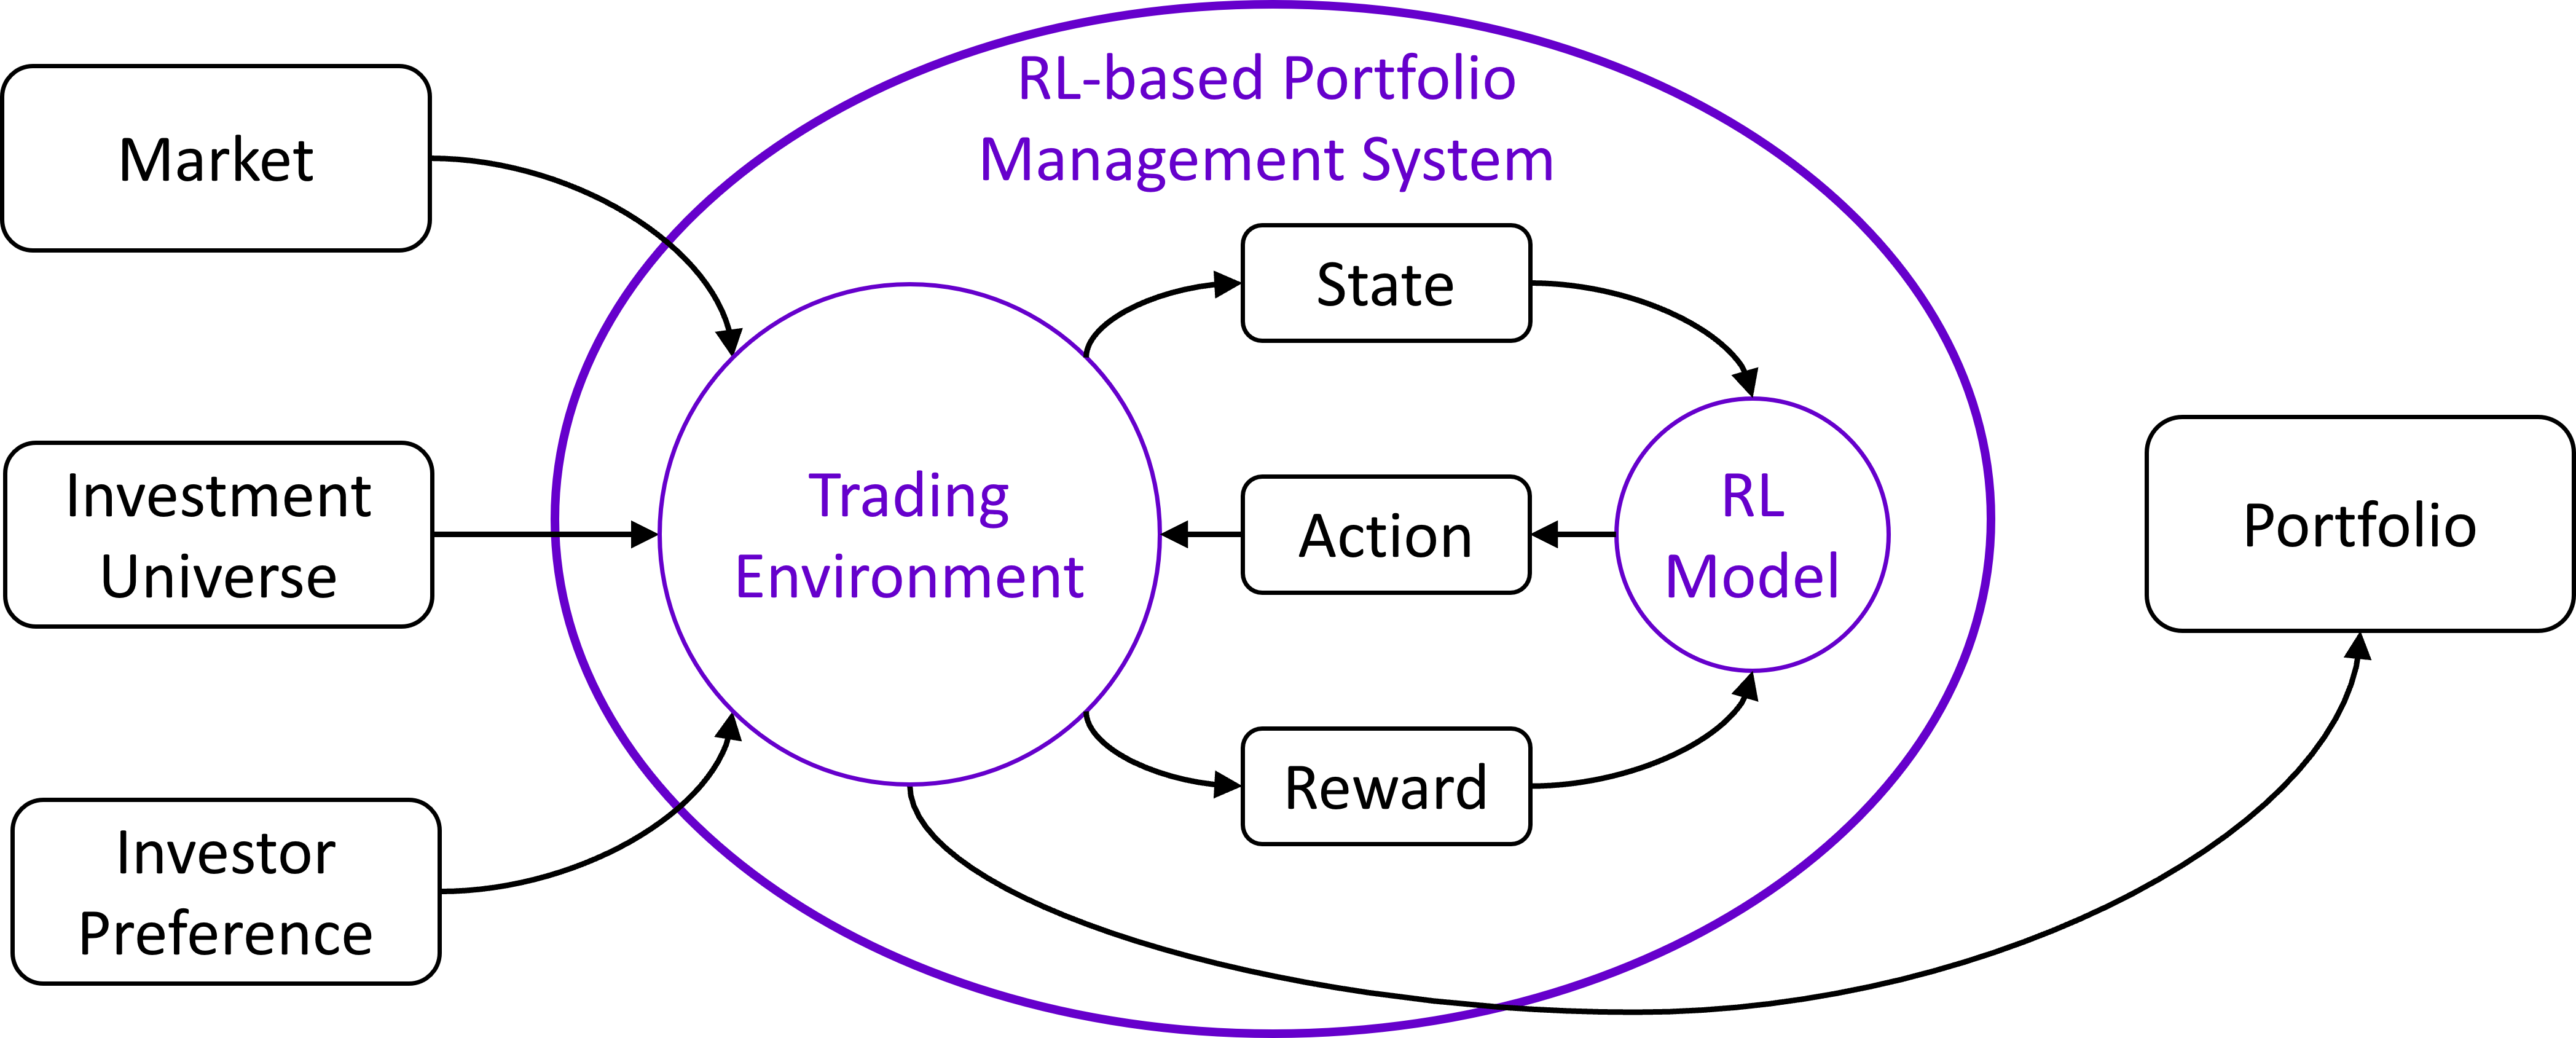
\includegraphics[width=15cm]{images/context_diagram.png}
  \caption{Context Diagram}
  \label{fig:context_diagram}
\end{figure}
\par
The RL-based Portfolio Management System contains two main parts, the training environment and the RL model. The trading environment bridges domain-specific inputs/outputs with the general-purpose RL model. This architecture enables the system to output the portfolio based on the inputs, the market, the investments, and the investor preference with most existing RL models.
